\chapter{Implementasi dan Pengujian}

\section{Implementasi Modul Aplikasi Android (Paket A)}
Pada sisi aplikasi Android (\texttt{app/src/main/java/coneckin/id/biz/id/}), implementasi difokuskan pada pemenuhan operasi CRUD penuh dan peningkatan keterujian kode (\textit{testability}):
\begin{itemize}[leftmargin=*]
  \item \textbf{Pemisahan Logika Murni:} Logika pengelolaan akun, pemetaan galat login, pemilihan portal, cache konfigurasi, dan antrean laporan dipisahkan ke dalam \texttt{AccountRepository.kt}, \texttt{LoginMapping.kt}, \texttt{PortalSelection.kt}, \texttt{Models.kt}, \texttt{Remote.kt}, dan \texttt{Reporter.kt} sehingga dapat diuji cepat di JVM.
  \item \textbf{Fitur Ubah Akun:} Layar utama pada \texttt{MainActivity.kt} dilengkapi ikon sunting pada setiap kartu akun yang membuka dialog \textit{Ubah Akun} terisi data lama untuk memperbarui nama akun, kredensial, dan daftar portal secara aman melalui \texttt{AccountStore}.
  \item \textbf{Konfigurasi JaCoCo:} Berkas \texttt{app/build.gradle.kts} menambahkan task \texttt{createDebugUnitTestCoverageReport} dan \texttt{verifyLogicCoverage} dengan batas minimal \textit{line coverage} sebesar 80\% pada modul logika inti.
\end{itemize}

\section{Implementasi Layanan API Server (Paket B)}
Pada direktori \texttt{server/}, kode monolitik dipecah menjadi tiga modul terstruktur:
\begin{itemize}[leftmargin=*]
  \item \textbf{\texttt{lib.js}:} Menyediakan validator \texttt{normalizeHost}, \texttt{isValidObjectId}, \texttt{parseReport}, \texttt{parsePortalCreate}, \texttt{parsePortalUpdate}, \texttt{parseConfigUpdate}, \texttt{parseReportQuery}, \texttt{summarizeReports}, \texttt{redact}, \texttt{rateLimit}, \texttt{requireAdmin}, dan \texttt{publicCors}.
  \item \textbf{\texttt{app.js}:} Pabrik aplikasi \texttt{createApp(...)} berbasis injeksi dependensi serta fungsi inisialisasi indeks dan data awal \texttt{prepareDatabase(database)}.
  \item \textbf{\texttt{server.js}:} Titik masuk produksi yang menghubungkan MongoDB (\texttt{DB\_NAME=coneckin\_db}), mengelola cache rilis GitHub selama 10 menit, dan menjalankan server HTTP Express 5.
\end{itemize}

\section{Implementasi Landing Page Croot.js (Paket C)}
Repositori \texttt{coneckin.github.io} diimplementasikan menggunakan konvensi modular ES6 Croot.js dengan struktur berikut:
\begin{itemize}[leftmargin=*]
  \item \texttt{js/croot.js}: Titik masuk modul utama yang menginisialisasi pengatur tema dan pemuatan data paralel.
  \item \texttt{js/config/url.js}: Konstanta endpoint produksi Alwaysdata, tautan rilis GitHub, dan direktori cadangan lokal (\texttt{ULBI — ypbpi.hotspot}).
  \item \texttt{js/lib/api.js} dan \texttt{js/lib/dom.js}: Utilitas \texttt{fetch} dengan \textit{timeout} 8 detik, validasi URL APK resmi, serta manipulasi DOM bebas XSS.
  \item \texttt{js/controller/landing.js} dan \texttt{js/controller/theme.js}: Memuat \texttt{GET /config}, \texttt{GET /portals}, dan \texttt{GET /health} secara paralel, menyediakan pencarian portal \textit{real-time}, tombol salin host, mode cadangan otomatis saat server tidak terjangkau, serta tombol ganti tema terang/gelap.
\end{itemize}

\section{Hasil Pengujian Otomatis dan Code Coverage}
Pengujian dilakukan pada tiga lapisan berbeda: pengujian unit JVM Android, pengujian instrumentasi pada emulator Android (\texttt{Medium\_Phone(AVD) - 17}), serta pengujian unit dan integrasi HTTP pada server Node.js. Ringkasan hasil pengujian ditampilkan pada Tabel~\ref{tab:hasil-uji}.

\begin{table}[H]
\centering
\caption{Rekapitulasi Hasil Pengujian Otomatis dan Code Coverage Ekosistem Coneckin}
\label{tab:hasil-uji}
\begin{tabular}{@{}p{4.4cm}ccc@{}}
\toprule
\textbf{Lapisan Pengujian} & \textbf{Jumlah Skenario} & \textbf{Line Coverage} & \textbf{Status} \\
\midrule
Android JVM Unit Test (JaCoCo) & 78 tes & 95,80\% (251/262 baris) & LULUS \\
Android Instrumented Test (\texttt{AndroidKeyStore}) & 11 tes & Terverifikasi AVD & LULUS \\
Server API Express (\texttt{app.js} + \texttt{lib.js}) & 39 tes & 96,53\% & LULUS \\
\midrule
\textbf{Total Pengujian Otomatis} & \textbf{128 tes} & \textbf{$>$ 95\%} & \textbf{LULUS} \\
\bottomrule
\end{tabular}
\end{table}

Rincian cakupan pengujian pada tiap lapisan meliputi:
\begin{enumerate}[leftmargin=*]
  \item \textbf{Android JVM Unit Test (78 tes):} Meliputi \texttt{AccountOpsTest}, \texttt{AccountRepositoryTest}, \texttt{LoginMappingTest}, \texttt{PortalSelectionTest}, \texttt{RemoteCacheStoreTest}, \texttt{ReportQueueTest}, serta rangkaian tes bawaan (\texttt{ModelsTest}, \texttt{RemoteTest}, \texttt{ReporterTest}). Seluruhnya lulus dengan cakupan 95,80\% sehingga jauh melampaui syarat minimal 80\%.
  \item \textbf{Android Instrumented Test (11 tes):} Dijalankan melalui \texttt{./gradlew connectedDebugAndroidTest} pada emulator Android (selesai dalam 19 detik, \texttt{BUILD SUCCESSFUL}). Pengujian mencakup 8 skenario pada \texttt{CryptoManagerInstrumentedTest} (enkripsi-dekripsi AES-256 GCM, keunikan IV acak, deteksi modifikasi \textit{ciphertext}, dan penanganan input tidak valid), 2 skenario pada \texttt{AccountStoreInstrumentedTest} (siklus simpan, baca, ubah, dan hapus akun terenkripsi), serta 1 skenario \texttt{ExampleInstrumentedTest}.
  \item \textbf{Server API Node.js (39 tes):} Meliputi \texttt{server/test/lib.test.js} dan \texttt{server/test/app.test.js} menggunakan injeksi basis data tiruan dalam memori. Seluruh jalur publik, validasi galat (\texttt{400}, \texttt{401}, \texttt{404}, \texttt{409}, \texttt{413}, \texttt{429}, \texttt{500}, \texttt{503}), otorisasi token admin, CRUD penuh (\texttt{portals}, \texttt{config}, \texttt{reports}), serta header CORS teruji dengan cakupan baris 96,53\%.
\end{enumerate}

\section{Verifikasi CI/CD dan Produksi End-to-End}
Setelah seluruh perubahan digabungkan ke cabang \texttt{main} pada repositori \texttt{coneckin} dan berkas server terbaru diunggah ke direktori kerja Alwaysdata (\texttt{/home/panlink/www/panlink-api}) dengan variabel lingkungan \texttt{MONGODB\_URI}, \texttt{DB\_NAME=coneckin\_db}, dan \texttt{ADMIN\_TOKEN}, dilakukan verifikasi langsung di lingkungan produksi:
\begin{itemize}[leftmargin=*]
  \item \textbf{GitHub Actions:} Alur kerja \texttt{Build and Release} dan \texttt{Server test} berstatus hijau serta menerbitkan rilis \texttt{v1.0.16} (\texttt{coneckin.apk} dan \texttt{coneckin.aab}).
  \item \textbf{Endpoint Kesehatan Produksi:} Permintaan \texttt{GET https://panlink.alwaysdata.net/health} mengembalikan status \texttt{HTTP 200 OK}, header \texttt{Access-Control-Allow-Origin: *}, serta muatan JSON \texttt{\{"ok":true,"db":true\}}.
  \item \textbf{Sinkronisasi Landing Page:} Halaman \url{https://coneckin.github.io/} menampilkan lencana versi terbaru (\texttt{v1.0.16}), lencana status hijau (\texttt{Server API \& Database Aktif}), direktori portal aktif dari server (\texttt{ULBI — ypbpi.hotspot}), dan tautan unduhan langsung APK terbaru.
\end{itemize}

% Catatan: Tambahkan bukti tangkapan layar ke folder images/ lalu aktifkan blok gambar berikut.
% \begin{figure}[H]
%   \centering
%   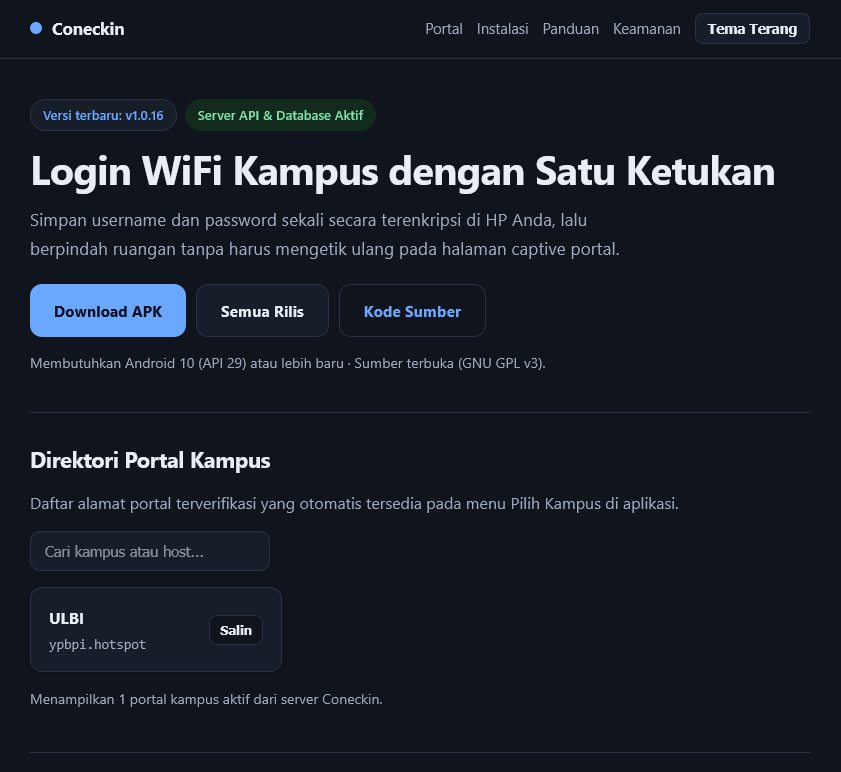
\includegraphics[width=0.92\textwidth]{images/landing-page-live.png}
%   \caption{Tampilan Landing Page \texttt{coneckin.github.io} terhubung aktif dengan API Alwaysdata.}
%   \label{fig:landing-live}
% \end{figure}
